\thispagestyle{duongvaotoanhocnone}
\pagestyle{duongvaotoanhoc}
\everymath{\color{duongvaotoanhoc}}
\graphicspath{{../duongvaotoanhoc/pic/}}
%\blfootnote{$^1$\text{.}}
\begingroup
\AddToShipoutPicture*{\put(0,616){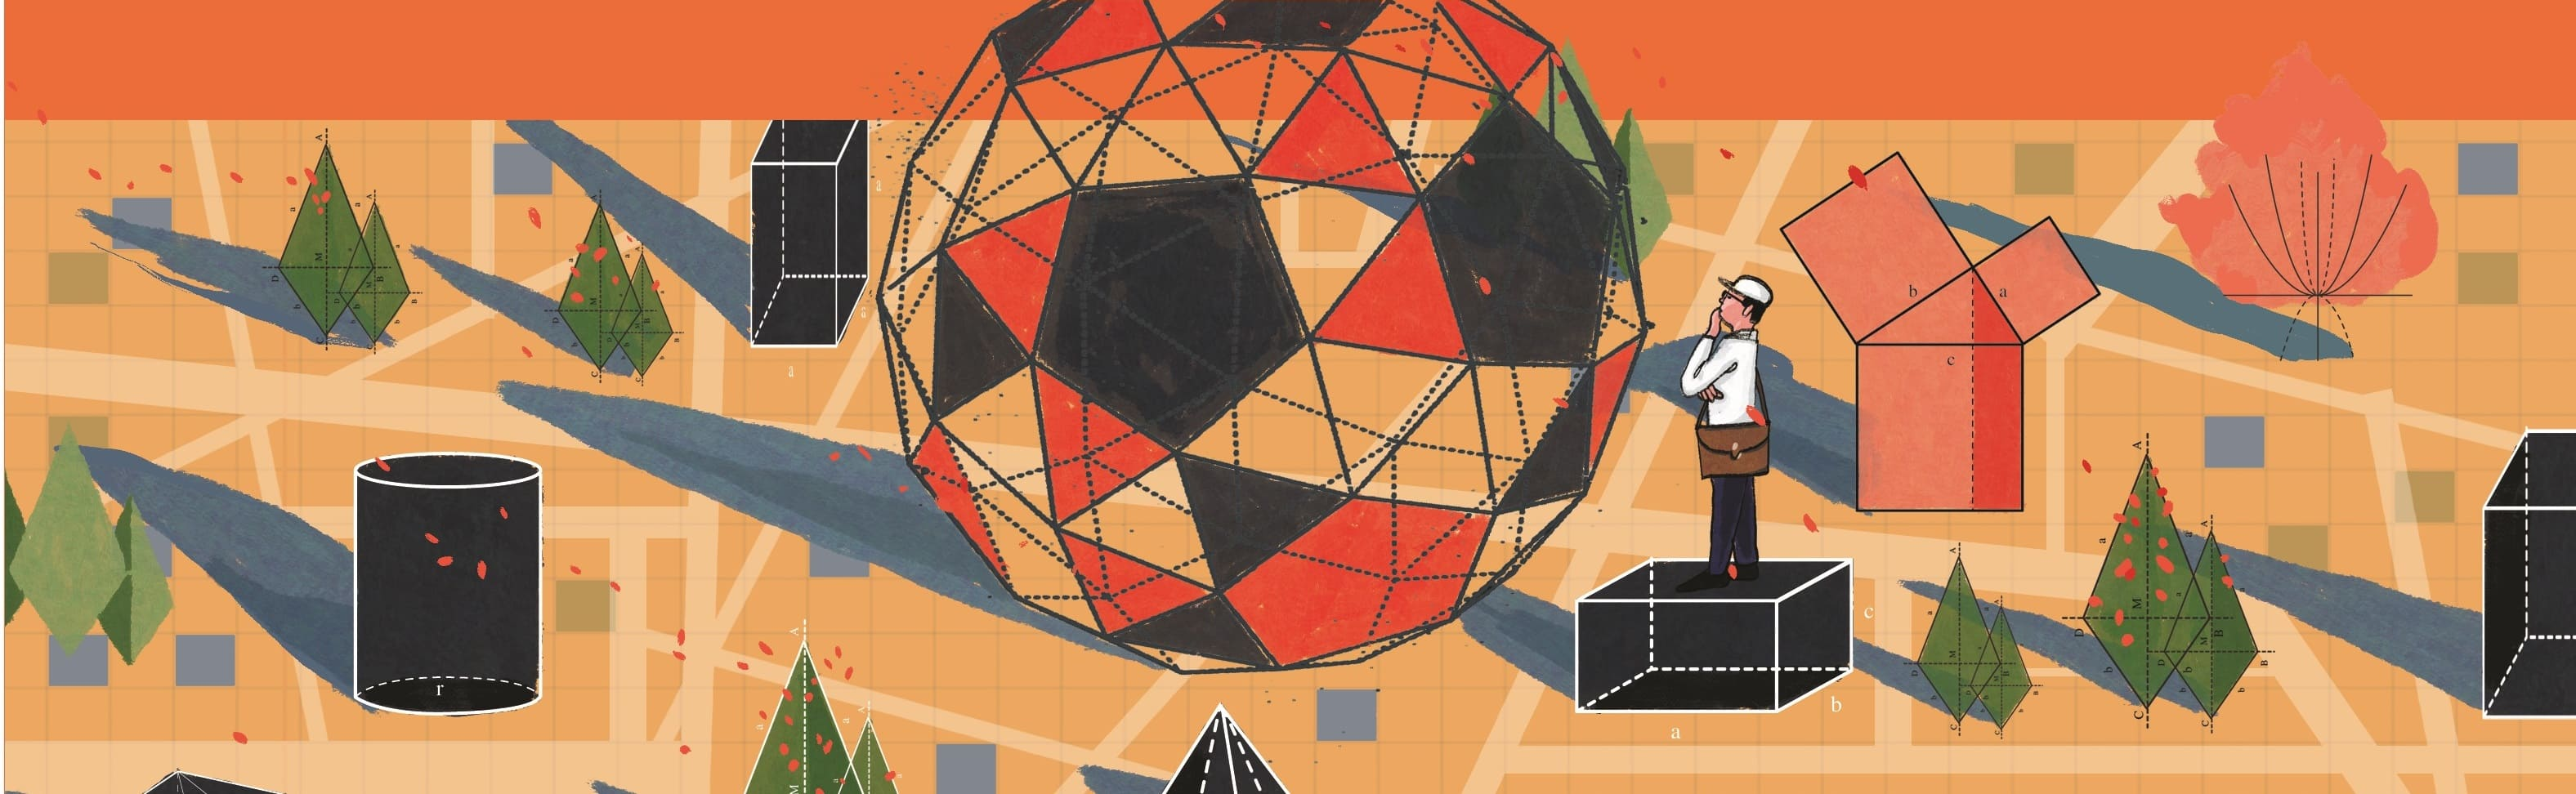
\includegraphics[width=19.3cm]{../bannerduongvao}}}
%\AddToShipoutPicture*{\put(138,522){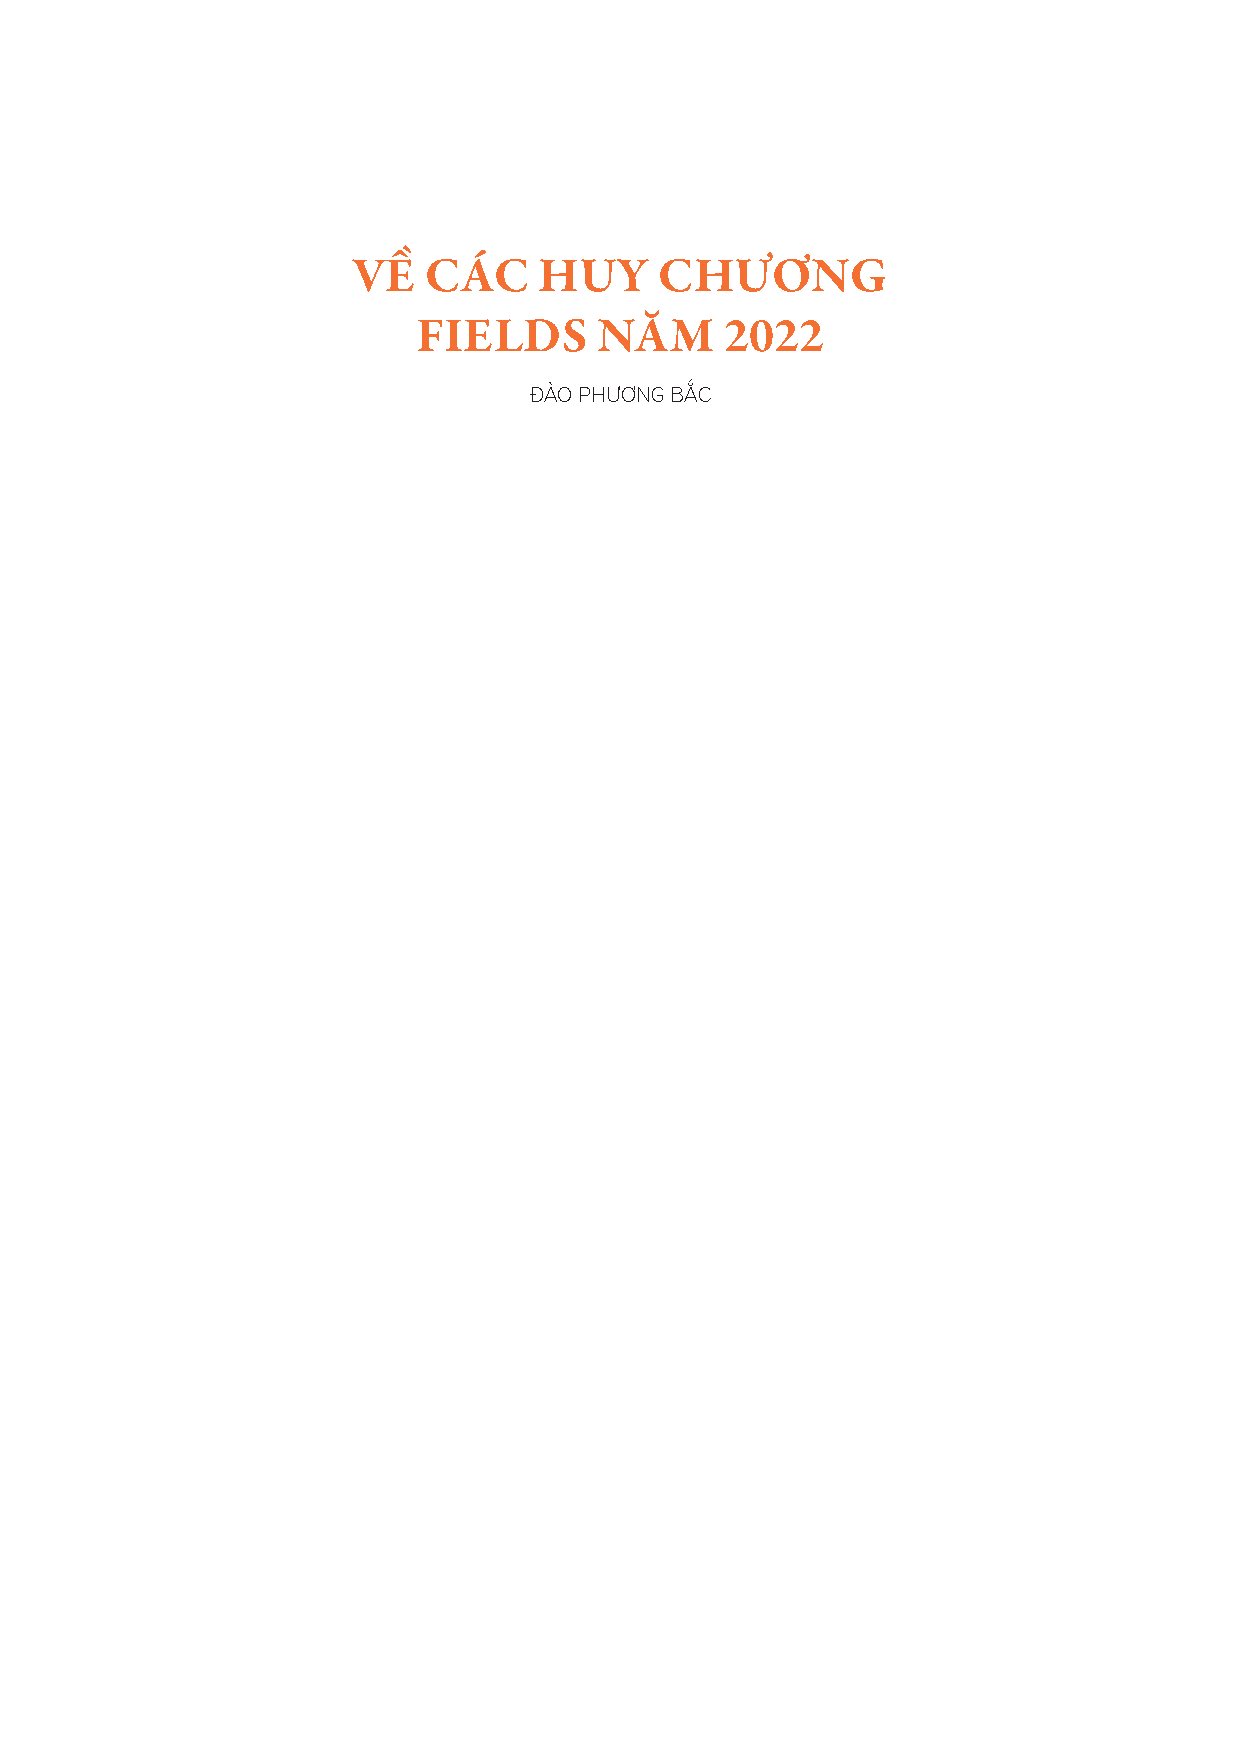
\includegraphics[scale=1]{../tieude.pdf}}}
\AddToShipoutPicture*{\put(130,522){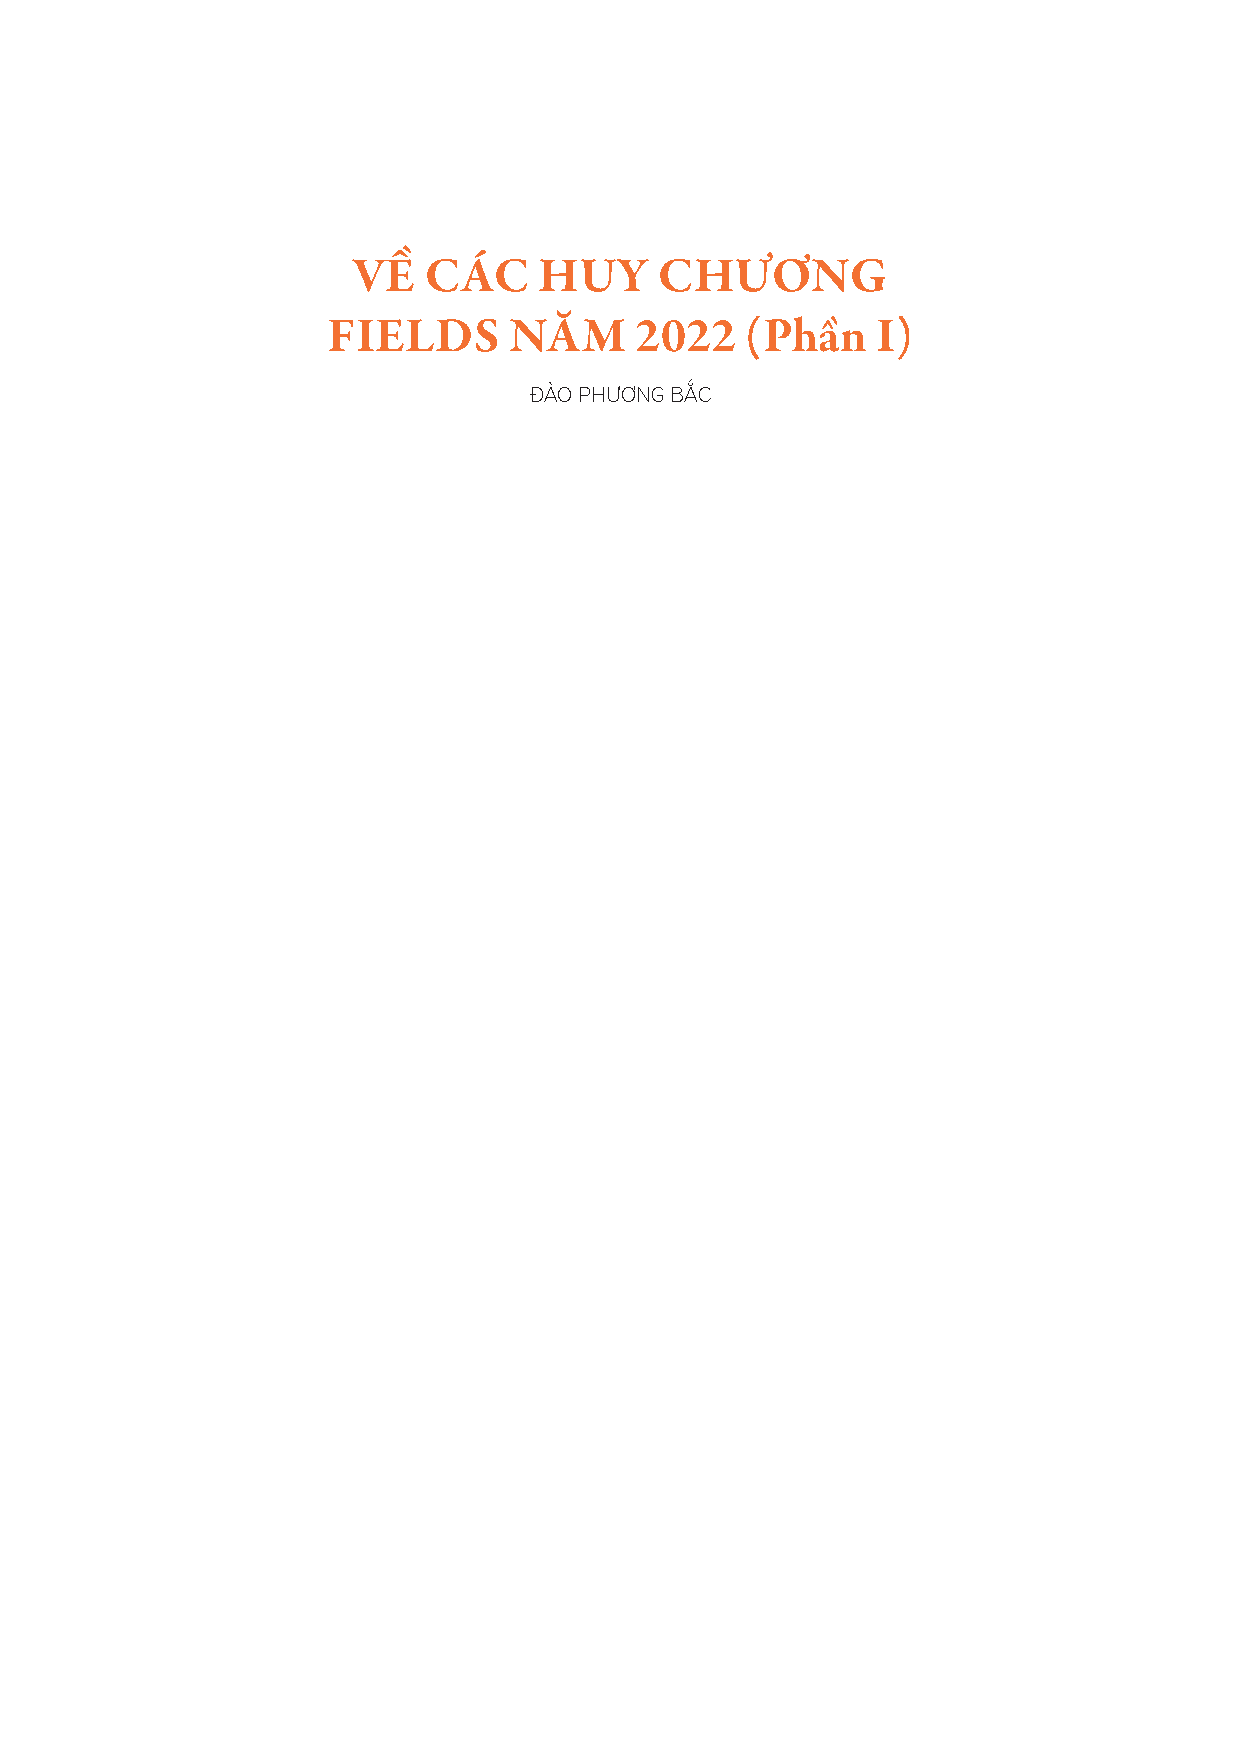
\includegraphics[scale=1]{../tieude1.pdf}}}
\centering
\endgroup

\vspace*{185pt}

\begin{multicols}{2}	
%	Đại hội Toán học thế giới (The International Congress of Mathematicians (ICM)) được tổ chức $4$ năm một lần là một sự kiện quan trọng của cộng đồng Toán học. Sau ``chiến dịch tranh cử'' của những nhà toán học Nga đứng đầu là hai Huy chương Fields A.~Okounkov và S.~K.~Smirnov, nước Nga đã giành quyền đăng cai. Nơi tổ chức Đại hội đã được ấn định từ trước là thành phố cổ kính Saint Petersburg từ ngày $6$ đến $14$ tháng $7$ năm $2022$. Tuy nhiên, vì một số yếu tố chính trị liên quan đến cuộc chiến giữa Nga và Ucraina, phiên họp trực tiếp đã không diễn ra, thay vào đó các báo cáo khoa học được để  dưới hình thức trực tuyến. Mặc dù vậy phiên họp Đại hội đồng của Liên đoàn Toán học thế giới nhằm bầu ra những vị trí chủ chốt của Liên đoàn Toán học thế giới nhiệm kỳ tiếp theo vẫn được tiến hành trực tiếp ở thủ đô Helsinki của Phần Lan với sự có mặt của các Chủ tịch hội toán học các nước. Tại phiên họp này các Huy chương Fields đã được trao vào ngày $5$ tháng $7$. Thực tế Helsinki cũng là nơi đăng cai Đại hội Toán học thế giới năm $1978$. Như chúng ta đã biết, ngoài điều kiện không quá $40$ tuổi, tiêu chí của Huy chương Fields là ``trao cho những khám phá xuất sắc trong Toán học đối với những công trình đặc biệt thú vị và hứa hẹn những khám phá tiếp theo''. Kết quả là $4$ Huy chương Fields năm $2022$ đã được trao cho các nhà toán học tài năng sau đây (lần lượt theo vần chữ cái): 
%	\vskip 0.1cm
%	$\bullet$ Hugo Duminil--Copin: Anh sinh năm $1985$ tại Pháp, là giáo sư tại Đại học Geneva, Thụy Sĩ, đồng thời cũng là giáo sư của Viện nghiên cứu cao cấp về Khoa học tự nhiên (Institut des Hautes Études Scientifiques--IHES), Cộng hòa Pháp . Anh được trao Huy chương Fields vì đã ``đã giải quyết những giả thuyết đã có từ lâu trong lý thuyết xác suất của hiện tượng chuyển pha trong Vật lý thống kê, đặc biệt là với số chiều $3$ và chiều~$4$".
%	\begin{figure}[H]
%		\centering
%		\vspace*{-5pt}
%		\captionsetup{labelformat= empty, justification=centering}
%		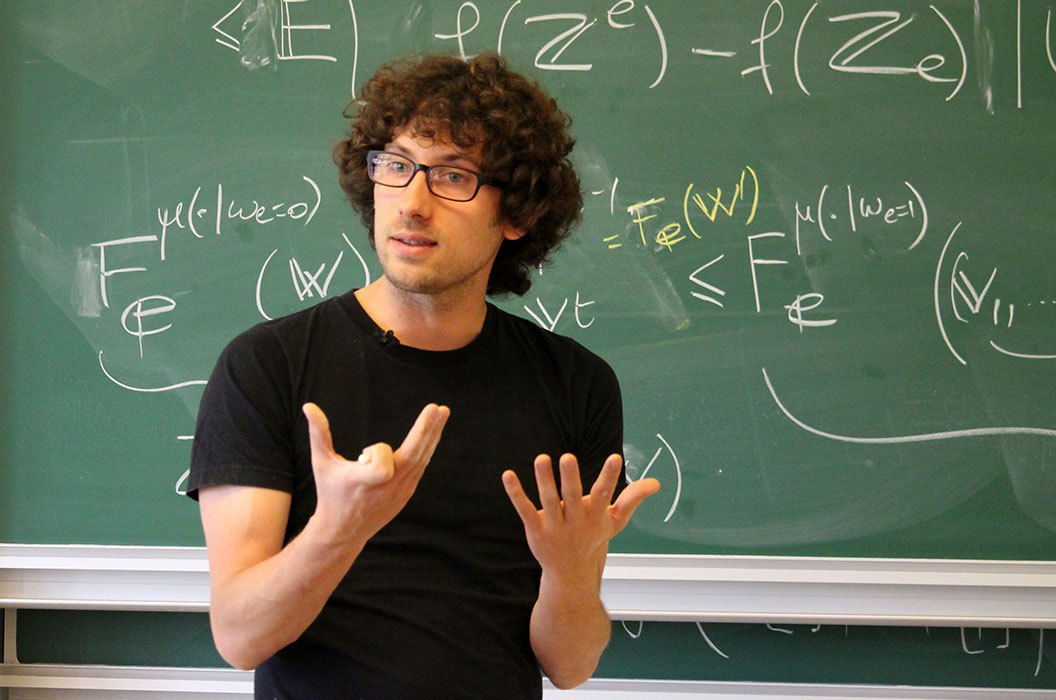
\includegraphics[width=1\linewidth]{Duminil-Copin}
%		\caption{\small\textit{\color{duongvaotoanhoc}Hugo Duminil--Copin.}}
%		\vspace*{-12pt}
%	\end{figure}
%	$\bullet$ June Huh: Anh sinh năm $1983$ tại Mỹ, nhưng là người Hàn Quốc và lớn lên cũng tại Hàn Quốc. Hiện anh là giáo sư tại Đại học\, Princeton,\, Hoa\, Kỳ.\, Anh\, nhận\, được\, Huy 
%	\end{multicols}
%	\begin{multicols}{2}
%	chương Fields vì ``việc mang những ý tưởng của lý thuyết Hodge vào tổ hợp, vì chứng minh giả thuyết Dowling--Wilson về các dàn hình học, chứng minh giả thuyết Heron--Rota--Welsh cho các matroids, và phát triển lý thuyết về các đa thức Lorentz, cùng với việc chứng minh giả thuyết Mason dạng mạnh".
%	\begin{figure}[H]
%		\centering
%		\vspace*{-5pt}
%		\captionsetup{labelformat= empty, justification=centering}
%		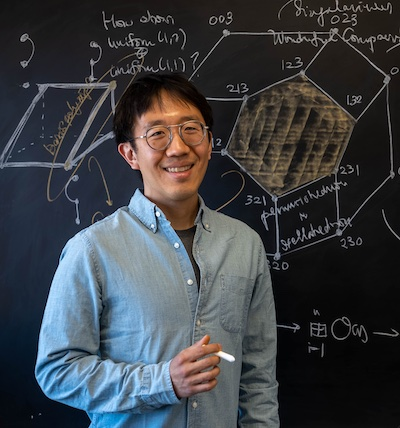
\includegraphics[width=1\linewidth]{Huh}
%		\caption{\small\textit{\color{duongvaotoanhoc}June Huh.}}
%		\vspace*{-10pt}
%	\end{figure}	
%	$\bullet$ James Maynard: Anh sinh năm $1987$ tại Vương Quốc Anh, là giáo sư tại Đại học Oxford. Huy chương Fields của J. Maynard
%	được trao cho việc đã có ``những đóng góp trong Lý thuyết số giải tích, dẫn đến những tiến bộ chính trong việc hiểu cấu trúc các số nguyên tố và trong xấp xỉ Diophantine". 
%	\vskip 0.1cm
%	$\bullet$ Maryna Viazovska: Chị sinh năm $1984$ tại Ucraina, là giáo sư đặc biệt (lãnh đạo nhóm Lý thuyết số) tại Đại học Bách Khoa Lausanne (EPFL), Thụy Sĩ. Chị được Huy chương Fields vì ``đã chứng minh được dàn $E_{8}$ cung cấp cách sắp xếp các hình cầu giống nhau một cách dày đặc nhất trong không không gian $8$ chiều, và những ứng dụng khác cho bài toán cực trị trong giải tích Fourier".
%	\vskip 0.1cm
%	Sau đây là một vài điểm chi tiết hơn một chút về công trình cũng như một vài thông tin khác của những nhà toán học nói trên. 
%	\begin{figure}[H]
%		\centering
%		\vspace*{5pt}
%		\captionsetup{labelformat= empty, justification=centering}
%		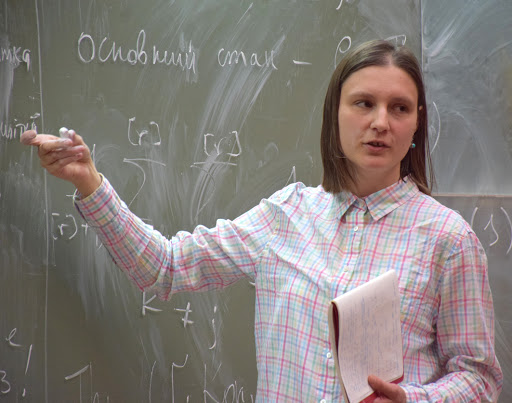
\includegraphics[width=1\linewidth]{Viazovska}
%		\caption{\small\textit{\color{duongvaotoanhoc}Maryna Viazovska.}}
%		\vspace*{-10pt}
%	\end{figure}
%	$1.$ Hugo Duminil--Copin: Anh được xem là đã làm thay đổi nền tảng toán học của hiện tượng chuyển pha trong Vật lý thống kê và đã giải quyết một số vấn đề mở đã có từ lâu trong Lý thuyết này, nói riêng trong trường hợp chiều $3$, chiều $4$ và trường hợp không khả tích khi số chiều bằng $2$. Chuyển pha là là một thuật ngữ mô tả sự chuyển tiếp các trạng thái của vật chất như rắn, lỏng, khí, plasma (ví dụ khi đun sôi đến $100$ độ C, dưới áp suất thông thường thì nước bắt đầu bay hơi). Mô hình Vật lý để mô tả những hiện tượng này là mô hình của E. Ising (một nhà Vật lý người Đức) trong Vật lý thống kê. Số chiều $2,3,4$ nói ở trên là số chiều của mô hình Ising. Công việc của Hugo Duminil--Copin là sự tiếp nối từ công việc của người thầy hướng dẫn của anh, Stanislav Smirnov (Huy chương Fields năm $2010$ về những đóng góp trong trường hợp số chiều $2$), cho những nền tảng toán học chặt chẽ để giải thích cho hiện tượng chuyển pha trong Vật lý nói trên thông qua mô hình Ising. Thực ra kết quả Toán học quan trọng đầu tiên về những mô hình Ising đã được L. Onsager (nhà bác học được giải Nobel về Hóa học năm $1968$) tìm ra. 
%	\vskip 0.1cm
%	Cần nói thêm rằng ngay từ khi làm luận án Tiến sĩ, Hugo đã có công trình quan trọng với thầy của mình giải quyết giả thuyết Nienhuis trong Vật lý thống kê về những hằng số liên kết cho những dàn lục giác. Chính kết quả này cũng đã góp phần tạo nên Huy chương Fields năm $2010$ của Stanislav Smirnov. Sau khi bảo vệ luận án Tiến sĩ năm $2013$, anh đã nhanh chóng trở thành chuyên gia hàng đầu về các khía cạnh xác suất của mô hình Ising. Bên cạnh mô hình Ising, Hugo còn có nhiều đóng góp cho mô hình Potts cũng trong Vật lý thống kê. Ở đây anh cùng với các cộng sự cũng đã giải quyết được một giả thuyết của Baxter đưa ra từ những năm $1970$. Vì những kết quả xuất sắc kể trên, khi chỉ ở độ tuổi $30$ anh đã là Giáo sư ĐH Geneve (Thụy Sĩ) và là Giáo sư ở Viện nghiên cứu cao cấp (Institut des Hautes Études Scientifiques (IHÉS)), Cộng hòa Pháp. Trước khi được trao Huy chương Fields, anh đã nhận được nhiều giải thưởng quan trọng như Giải thưởng của Hội Toán học Châu Âu, Giải thưởng của Viện hàn lâm khoa học Pháp, và một số giải thưởng của chuyên ngành Xác suất như giải thưởng Loeve, Dobrushin, ...  
%	\vskip 0.1cm
%	$2.$ James Maynard: Các công việc của anh được xem có tính độc đáo rất cao, thường dẫn đến những kết quả có tính đột phá đáng ngạc nhiên cho những vấn đề quan trọng, tưởng chừng như không thể thực hiện được với những kỹ thuật hiện tại.  
%	\begin{figure}[H]
%		\centering
%		\vspace*{-5pt}
%		\captionsetup{labelformat= empty, justification=centering}
%		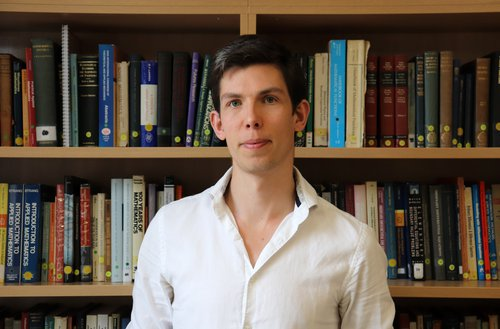
\includegraphics[width=1\linewidth]{Maynard}
%		\caption{\small\textit{\color{duongvaotoanhoc}James Maynard.}}
%		\vspace*{-10pt}
%	\end{figure}
%	Anh là một nhà Toán học người Anh, và được phong giáo sư ở Đại học Oxford danh tiếng vào năm $2017$ khi mới vừa tròn $30$ tuổi. Trước đó, anh làm dưới sự hướng dẫn của một trong những chuyên gia đầu ngành về Lý thuyết số giải tích là Roger Heath--Brown. Trước khi được trao Huy chương Fields, anh đã dành được một số giải thưởng quan trọng khác như giải thưởng SASTRA Ramanujan năm $2014$, giải thưởng Whitehead cho các nhà toán học trẻ của Hội Toán học London năm $2015$, giải thưởng của Hội toán học Châu Âu năm $2016$.    
%	\vskip 0.1cm
%	Như đã biết, số nguyên tố là một lĩnh vực cổ điển của Lý thuyết số mà không nhiều người dám thử sức vì khả năng có kết quả tương đối thấp. Ngoại trừ kết quả về vô hạn số nguyên tố có từ thời Eulid, mà chứng minh của nó chỉ vài dòng được giới thiệu trong chương trình cấp hai, thì các kết quả được xem là định lý về số nguyên tố đều có các chứng minh ít nhiều cần đến kiến thức ở bậc đại học trở lên và rất khó. Ở góc nhìn tổng thể về phân bố số nguyên tố, một trong những kết quả quan trọng mở đầu cho những ứng dụng của giải tích trong số nguyên tố là định lý của J. Hadamard và de vallee Poussin năm $1896$ (được dự đoán từ trăm năm trước đó bởi A--M. Legendre):
%	\vskip 0.1cm
%	\textbf{\color{duongvaotoanhoc}Định lý} $\pmb{1.}$ \textit{Với $\pi(n)$ là số lượng các số nguyên tố nhỏ hơn hay bằng $n$ thì} 
%	\begin{align*}
%		\lim_{n \to \infty} \frac{\pi(n)}{{\rm ln}n}=1.
%	\end{align*}
%	Liên quan đến phân bố các số nguyên tố thì dự đoán lớn nhất còn tồn tại có lẽ là giả thuyết Riemann về không điểm của hàm zeta. Bên cạnh đó, một mặt với số $n$ lớn tùy ý luôn tồn tại một dãy $n$ số liên tiếp gồm toàn hợp số (chẳng hạn $(n+1)!+2, (n+1)!+3, \ldots, (n+1)!+(n+1)$), nhưng {\it có thể có} những cặp số nguyên tố sinh đôi $(p,p+2)$ lớn tùy ý, chẳng hạn $(518807,518809)$. Đó chính là nội dung của câu hỏi về cặp số nguyên tố sinh đôi vẫn còn mở: 
%	\vskip 0.1cm
%	\textbf{\color{duongvaotoanhoc}Câu hỏi} $\pmb{1.}$
%		Tồn tại vô hạn cặp số nguyên tố sinh đôi $(p,p+2)$?
%	\vskip 0.1cm
%	Năm $2006$, một kết quả quan trọng theo hướng khẳng định giả thuyết về các cặp số nguyên tố sinh đôi của Goldston--Graham--Pintz--Yıldırım đã chỉ ra 
%	\vskip 0.1cm
%	\textbf{\color{duongvaotoanhoc}Định lý} $\pmb{2.}$ (Goldston--Graham--Pintz--Yıldırım, Proc. Japan Academy $2006$).
%	\textit{Ký hiệu $p_{n}$ là số nguyên tố thứ $n$ thì}
%	\begin{align*}
%		\liminf  \frac{p_{n+1}-p_{n}}{{\rm log}p_{n}}=0.
%	\end{align*}
%	Sau đó, vào năm $2013$ có một bước tiến rất ấn tượng của Y. Zhang như sau.
%	\vskip 0.1cm
%	\textbf{\color{duongvaotoanhoc}Định lý} $\pmb{3.}$ (Y. Zhang, Ann. Math. $179$ ($2014$), $1121$--$1174$).
%	\textit{Với một số $N$ nào đó nhỏ hơn $70$ triệu, tồn tại vô hạn cặp số nguyên tố sai khác $N$. }
%	\vskip 0.1cm
%	Cũng cần phải nói thêm Y. Zhang lúc đó chỉ là một giảng viên Toán bình thường ở Đại học New Hampshire. Đây không hẳn là một đại học nghiên cứu (có đào tạo bậc Tiến sĩ về Toán), ở vùng Đông Bắc nước Mỹ. Sở dĩ ông công tác ở một đại học nhỏ như vậy vì kết quả chính trong luận án Tiến sĩ của mình tuy được công bố ở một tạp chí uy tín cao là Duke Math. J. nhưng đã sử dụng một kết quả mà sau này người ta mới biết là sai. Tuy kết quả năm $2014$ của Y. Zhang rất ấn tượng nhưng sau đó đã được làm mạnh hơn rất nhiều bởi James Maynard và nhóm của T. Tao (một nhà toán học rất nổi tiếng, Huy chương Fields năm $2006$) và các cộng sự. Điển hình là kết quả sau giảm số $70$ triệu của định lý trước của Y. Zhang xuống còn $600$:
%	\vskip 0.1cm
%	\textbf{\color{duongvaotoanhoc}Định lý} $\pmb{4.}$ (James Maynard, Ann. Math. ($2015$), vol. $181$ (no.$1$) $383$--$413$, nhóm của T. Tao cũng cho một chứng minh độc lập).
%	\textit{Ký hiệu $p_{n}$ là số nguyên tố thứ $n$ thì}
%	\begin{align*}
%		\liminf (p_{n+1}-p_{n}) \leq 600. 
%	\end{align*}
%	\textit{Nếu thừa nhận giả thuyết Elliot--Halberstam thì} 
%	\begin{align*}
%		\liminf (p_{n+1}-p_{n}) \leq 12,
%	\end{align*}
%	\textit{và}
%	\begin{align*}
%		\liminf(p_{n+2}-p_{n}) \leq 600. 
%	\end{align*}
%	Phương pháp mà James Maynard sử dụng phát triển phương pháp ``sàng'' của nhóm tác giả D. A. Goldston, J. Pintz, C. Y. Yildirim (Ann. Math. $2009$). Gốc rễ của phương pháp này chính là sàng Eratosthenes có từ thời cổ đại dùng để lọc ra các số nguyên tố nhỏ hơn một số cho trước. Ngoài kết quả có tính đột phá kể trên, J. Maynard cũng đã có những đóng góp cơ bản trong xấp xỉ Diophantine, cùng với Koukoulopoulos anh đã giải quyết Giả thuyết Duffin--Schaeffer (Ann. Math $2020$). Giả thuyết này được đưa ra năm $1941$, mô tả việc một số thực có thể được xấp xỉ tốt bởi một số hữu tỷ đến mức độ nào, và bắt nguồn từ bổ đề xấp xỉ nổi tiếng của Dirichlet. 
%	\vskip 0.1cm
	$3.$ June Huh: Anh được xem là đã cùng với một số cộng sự làm thay đổi lĩnh vực hình học tổ hợp thông qua việc dùng các phương pháp của lý thuyết Hodge (phương pháp để nghiên cứu đối đồng điều của những đa tạp Kahler compact), hình học nhiệt đới (tropical), và lý thuyết kỳ dị. Đối tượng tổ hợp chính mà June Huh quan tâm là các matroids. Matroid là một đối tượng gần với ma trận (matrix) và lý thuyết đồ thị, và lý thuyết về chúng có cảm hứng từ việc trừu tượng hóa nhiều khái niệm từ hai lý thuyết nói trên. Cụ thể hơn, matroid $M$ là một cặp $(E,\pazocal{I})$ gồm một tập hữu hạn $E$ và một họ $\pazocal{I}$ khác rỗng các tập con của $E$ thỏa mãn đồng thời $2$ điều kiện:
	\vskip 0.1cm
	$\bullet$ Nếu tập con $A$ của $E$ thuộc họ $\pazocal{I}$ thì mọi tập con của nó cũng thuộc $\pazocal{I}$.
	\vskip 0.1cm
	$\bullet$ Nếu $A, B \in \pazocal{I}$ và $|A| = |B| +1$, thì tồn tại một phần tử $x \in A \setminus B$ sao cho $B \cup \{x\} \in \pazocal{I}$.
	\vskip 0.1cm
	Mô hình cụ thể của một matroid là một ma trận với các cột đánh số bởi tập $E$ và họ $\pazocal{I}$ các tập con mà các cột ứng với tập con đó là độc lập tuyến tính.
	\vskip 0.1cm
	Đây là một khái niệm đưa ra bởi một nhà hình học nổi tiếng của thế kỷ trước là H. Whitney sau đó được phát triển nhiều bởi một chuyên gia nổi tiếng về tổ hợp là G--C. Rota. Sau này matroids tìm thấy nhiều ứng dụng trong hình học, tôpô, tổ hợp, ...
	\vskip 0.1cm
	Bên cạnh đó, hình học nhiệt đới (tropical) là một biến thể của hình học đại số. Trong khi hình học đại số nghiên cứu những đa tạp đại số là tập nghiệm của một hệ phương trình đa thức thì hình học nhiệt đới thay phép cộng trong đa thức bởi phép lấy giá trị nhỏ nhất và phép nhân thay bằng phép cộng. Ngay trong hình học đại số, lý thuyết hình học mới này đã có nhiều ứng dụng thông qua các công trình của M. Kontsevich (Huy chương Fields năm $1998$) và G. Mikhalkin. Tuy xuất phát từ hình học đại số nhưng theo nhận xét của June Huh các đa tạp nhiệt đới rộng hơn nhiều so với việc lấy nhiệt đới hóa (tropicalization) các đa tạp đại số, qua đó cho thấy những nghiên cứu của June Huh chắc sẽ còn hứa hẹn nhiều kết quả quan trọng.  
	\vskip 0.1cm
	Cụ thể hơn những công trình quan trọng làm nên Huy chương Fields của June Huh bao gồm:
	\vskip 0.1cm
	$\bullet$ June Huh đã cùng với Boton Wang sử dụng Hình học đại số và lý thuyết giao để chứng minh giả thuyết Dowling--Wilson về nhận biết các matroids. 
	\vskip 0.1cm
	$\bullet$ Karim Adiprasito, June Huh, và Eric Katz đã tìm ra một dạng tương tự của lý thuyết Hodge và chứng minh định lý Lefschetz dạng mạnh và quan hệ Hodge--Riemann cho các matroids tùy ý. Họ đã dùng các kết quả này để giải quyết giả thuyết Heron--Rota--Welsh về tính lõm loga của đa thức đặc trưng của một matroid. 
	\vskip 0.1cm
	$\bullet$ Petter Branden và June Huh đã phát triển lý thuyết về các đa thức Lorentz, liên hệ với giải tích lồi và phiên bản rời rạc của nó thông qua hình học nhiệt đới. Họ đã chứng minh giả thuyết Mason dạng mạnh cho các matroids và tìm ra các ứng dụng khác nhau từ hình học đại số xạ ảnh cho tới mô hình Potts trong cơ học thống kê (đã được đề cập đến trong công việc của Hugo Duminil--Copin).
	\vskip 0.1cm 
	June Huh có một quá trình đào tạo về Toán không thật chính quy. Anh tự nhận không giỏi Toán khi học phổ thông và học cả chuyên ngành Vật lý ở bậc đại học ở Đại học Quốc Gia Seoul (Hàn Quốc) nhưng bảng điểm không thật tốt. Đến những năm cuối đại học, anh được tham dự các bài giảng về Hình học đại số của H. Hironaka (Huy chương Fields năm $1970$ của Nhật Bản, nổi tiếng với định lý giải kỳ dị) khi ông là Giáo sư mời của Đại học Quốc gia Seoul. Lúc này anh bắt đầu có cảm hứng và bắt đầu dành nhiều thời gian hơn cho Toán học. Tốt nghiệp Đại học xong, anh làm luận văn Thạc sĩ với một trong những chuyên gia hàng đầu về Hình học đại số của Hàn Quốc là Young--Hoon Kiem. Sau đó, năm $2009$, anh được nhận làm luận án Tiến sĩ Toán ở Mỹ, ban đầu là Đại học Illinois ở Urbana--Champaign, sau đó chuyển sang Đại học Michigan. Anh bảo vệ luận án Tiến sĩ năm $2014$ dưới sự hướng dẫn của một chuyên gia nổi tiếng về Hình học đại số là M. Mustata. Tuy bắt đầu làm luận án Tiến sĩ khá muộn, nhưng ngay từ những năm đầu khi làm luận án Tiến sĩ, anh đã dùng những kỹ thuật của hình học đại số để chứng minh giả thuyết Read về hệ số của đa thức sắc số (chromatic polynomials) trong lý thuyết đồ thị. Đây là một giả thuyết từ hơn $40$ năm trước xuất phát từ bài toán $4$ màu nổi tiếng mà lời giải của nó dài vài trăm trang được đưa ra bởi K. Appel và W. Haken năm $1976$ cùng với sự hỗ trợ của máy tính. Bài báo của June Huh ngay lập tức đã được chú ý và in ở một tạp chí hàng đầu là Journal of the American Mathematical Society. Một điều thú vị là chính trong bài báo này, June Huh cũng đã trả lời một câu hỏi liên quan của GS. Ngô Việt Trung và J. K. Verma về số bội trộn trong Đại số giao hoán. Nhờ những kết quả quan trọng trong luận án, anh được nhận học bổng nghiên cứu danh giá của Viện Clay, và nhận vị trí Veblen Instructor, cũng như vị trí giáo sư mời ở Viện nghiên cứu cao cấp Princeton. Đến năm $2020$, anh nhận vị trí giáo sư ở Đại học Stanford, nhưng chỉ $1$ năm sau đó anh quay lại nhận vị trí giáo sư ở Đại học Princeton.     
	\vskip 0.1cm
	$4.$ Maryna Viazovska: Như đã nói ở trên được trao huy chương Fields một phần vì những đóng góp trong bài toán xếp hình cầu.
	\vskip 0.1cm
	Một vấn đề có từ lâu trong toán học là tìm một cách sắp xếp dày đặc nhất (tối ưu nhất) những hình cầu giống nhau trong không gian với số chiều cho trước. Dày đặc nhất ở đây hiểu là tỷ lệ giữa tổng thể tích các hình cầu và thể tích hình chứa nó là lớn nhất. Bài toán này cũng rất tự nhiên trong thực tế khi ta đi du lịch và cần phải xắp xếp sao cho balo chứa được nhiều đồ vật nhất. Ở chiều $2$ ta biết cách sắp xếp theo hình lục lăng (một hình tròn ở giữa, $6$ hình tròn đặt xung quanh trong một lục giác đều) cho ta cách xếp dày đặc nhất. Với số chiều $3$, từ vài trăm năm trước, J. Kepler đã dự đoán cách xếp các quả cam chứa trong một hình kim tự tháp sẽ cho kết quả tối ưu. Năm $1998$, T. Hales chứng minh giả thuyết Kepler với một chứng minh gần $100$ trang in ở Annals of Mathematics cùng với sự trợ giúp của máy tính. Bài toán sắp xếp hình cầu không có thêm kết quả gì ở các số chiều khác cho đến năm $2016$, M.~Viazovska chỉ ra dàn $E_{8}$ (dàn (lưới) trong không gian $\mathbb{R}^8$, liên quan đến nhóm Lie dạng $E_{8}$) cho cách xếp tối ưu nhất trong chiều $8$. Ít lâu sau đó cùng với H. Cohn, A. Kumar, S. Miller và D. Radchenko, M.~Viazovska đã chứng minh dàn Leech cho cách sắp xếp dày đặc nhất ở số chiều $24$. Dàn Leech nằm trong không gian $\mathbb{R}^{24}$ có nhóm các tự đẳng cấu là nhóm đơn hữu hạn loại lẻ tẻ (sporadic) đưa ra bởi Conway. Lời giải của M.~Viazovska dựa trên cách tiếp cận của H. Cohn và N.~Elkies (Ann. Math. $2003$), những người đã dùng công thức tổng Poisson của giải tích điều hòa để tìm ra một chặn trên cho những khả năng có thể có của mật độ cho bài toán xếp cầu với số chiều tùy ý. Công trình của các nhà toán học này cần đến sự tồn tại của những hàm Schwatz với những tính chất đặc biệt (chẳng hạn hàm đó và biến đổi Fourier của nó triệt tiêu tại những giá trị độ dài của vectơ trong các dàn tương ứng). H. Cohn và N.~Elkies nghĩ rằng những hàm có tính chất đặc biệt như thế là tồn tại nhưng chưa có ý tưởng gì để xây dựng. Khi công việc dừng ở đó khoảng $10$ năm thì M.~Viazovska xuất hiện và đưa ra một phương pháp hoàn toàn mới để đưa ra những hàm này dựa trên lý thuyết về các dạng modular. Như chúng ta đã biết các dạng modular là một lĩnh vực thuộc Lý thuyết số hiện đại và cung cấp những điểm mấu chốt cho lời giải bài toán Fermat của A. Wiles từ khoảng gần $30$ năm trước. Sau đó kỹ thuật chọn hàm Schwatz dùng dạng modular cũng đã được H. Cohn khai thác và thu được những kết quả quan trọng gần đây. Việc dùng các dạng modular là một đối tượng rất khác để giải quyết vấn đề nói trên ít nhiều có sự hợp lý nếu chúng ta nhìn vào đào tạo của M.~Viazovska. Ngay từ phổ thông, chị đã là một học sinh giỏi Toán, tốt nghiệp Đại học ở Ucraina, sau đó làm luận văn cao học Đức, rồi quay lại Ucraina làm luận án Tiến sĩ và bảo vệ vào năm $2010$. Sau đó chị sang Đức làm luận án Tiến sĩ với một trong hai người thầy hướng dẫn là Don Zagier, một chuyên gia về nhiều thứ trong đó có lý thuyết các dạng modular. Một điều đáng ngạc nhiên là mặc dù lời giải bài toán xếp cầu trong trường hợp $3$ chiều rất dài và cần đến máy tính kiểm tra nhưng lời giải trong trường hợp $8$ chiều và $24$ chiều lại khá ngắn gọn (khoảng $20$ trang). Vì những kết quả độc đáo này, M.~Viazovska đã nhận được giải thưởng nghiên cứu của Viện Clay năm $2017$ dành cho những kết quả Toán học xuất sắc nhất trong năm.        
	\vskip 0.1cm
	Sau lời giải bài toán xếp cầu ở chiều $8$ và $24$, M.~Viazovska đã phát triển tiếp tục ý tưởng của riêng mình. Chị đã cùng với D.~Radchenko ($2019$) chứng minh mọi hàm Schwatz chẵn thỏa mãn hàm đó cùng với biến đổi Fourier triệt tiêu tại các số $\sqrt{n}$ ($n$ là số nguyên không âm) luôn đồng nhất bằng $0$. Kết quả này được các chuyên gia đánh giá là rất đáng ngạc nhiên.
	\vskip 0.1cm
	{\bf\color{duongvaotoanhoc} Kết luận:}  Từ những phân tích kể trên ta thấy đóng góp của những giải thưởng Fields luôn rất đặc biệt, thường là lời giải cho những vấn đề quan trọng, và lời giải nhiều khi đến từ những lĩnh vực hoàn toàn khác.
	\vskip 0.1cm
	\textbf{\color{duongvaotoanhoc}Tài liệu tham khảo}
	\vskip 0.1cm
	[$1$] Trang web \url{https://www.mathunion.org/imu-awards/fields-medal/fields-medals}\\ \url{-2022}
	\vskip 0.1cm
	[$2$] Các trang wikipedia.
\end{multicols}
